\documentclass[12pt,a4paper]{article}

\usepackage{graphicx}
\usepackage{geometry}

\geometry{margin=1in}

\title{Human Computer Interaction and Computer Graphics}
\author{Shiza Nizamani \\ Roll Number: 2k24/CSE/142}
\date{\today}

\begin{document}

\maketitle

\section{Introduction}

This assignment analyzes Human-Computer Interaction (HCI) and Computer Graphics (CG) from the user's perspective. The selected application is Spline, a web-based design tool that allows users to create interactive 3D and 2D web experiences directly in a browser without writing code. The HCI analysis focuses on the toolbar and editing section, which allow users to make interactive changes to objects. The CG analysis examines the perspective view of a 3D cube and the visual elements that contribute to its three-dimensional appearance. Finally, the report reflects on how graphics quality affects user interaction and identifies a simple HCI improvement that could enhance the user experience.

\section{HCI Analysis}

The Spline interface provides several interaction elements that allow users to create and modify objects within the 3D environment.

\begin{figure}[h]
    \centering
    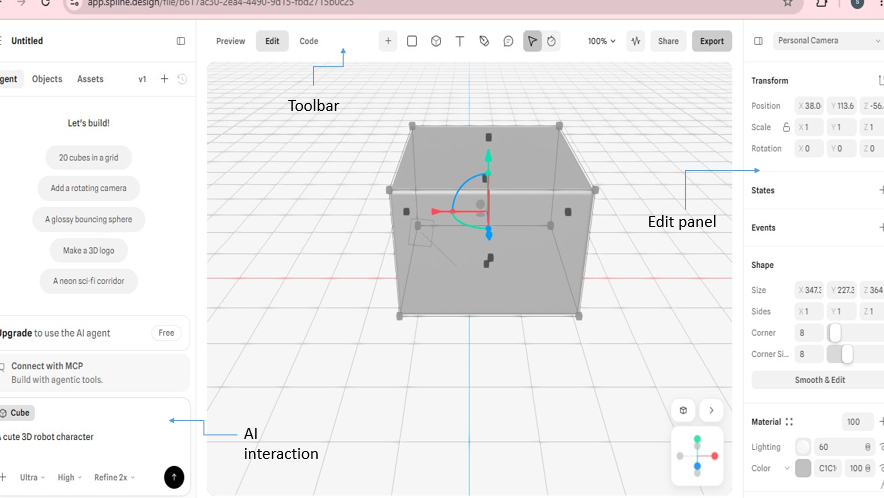
\includegraphics[width=0.9\textwidth]{HCI 1.png}
    \caption{Annotated screenshot of Spline interface showing HCI interaction elements.}
    \label{fig:hci}
\end{figure}

\subsection{HCI Interaction Elements}

\begin{enumerate}

    \item \textbf{Toolbar:}
    The toolbar provides users with tools for selecting and manipulating objects in the 3D environment. It supports direct interaction by allowing users to perform actions such as moving, rotating, and scaling objects.

    \item \textbf{Edit Panel:}
    The edit panel allows users to modify properties of the selected object. This gives users greater control over the appearance and characteristics of objects without requiring them to write code.

    \item \textbf{AI Interaction:}
    The AI section provides an alternative way for users to interact with the application through AI-assisted input. This can simplify the creation or modification of 3D content, particularly for users who may not be familiar with traditional 3D design tools.

\end{enumerate}

\section{CG Analysis}

The Spline 3D environment uses different visual and rendering elements to represent objects and create a sense of three-dimensional space. The selected cube demonstrates perspective, three-dimensional geometry, and material appearance.

\begin{figure}[h]
    \centering
    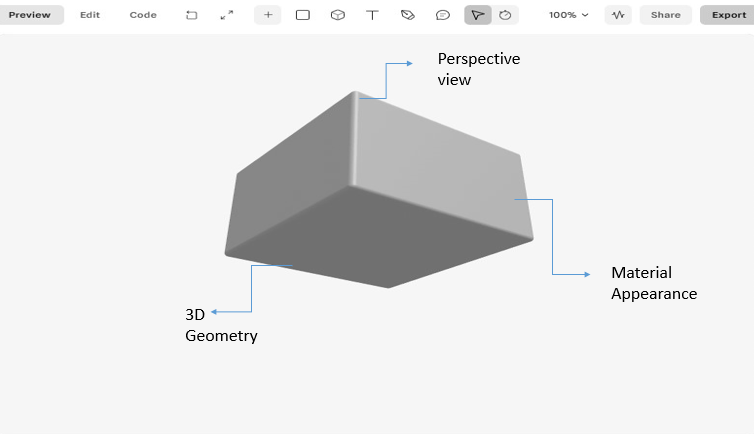
\includegraphics[width=0.9\textwidth]{CG 1.png}
    \caption{Annotated screenshot of the Spline 3D environment showing CG visual elements.}
    \label{fig:cg}
\end{figure}

\subsection{CG Visual Elements}

\begin{enumerate}

    \item \textbf{Perspective View:}
    The perspective view represents objects in a way that provides a sense of depth. Objects and surfaces that are farther from the viewer appear smaller, which helps create a realistic three-dimensional spatial representation.

    \item \textbf{3D Geometry:}
    The cube is represented using three-dimensional geometry consisting of multiple faces and edges. This geometry gives the object its physical 3D shape and allows it to be viewed from different angles.

    \item \textbf{Material Appearance:}
    The material appearance defines how the surface of the cube looks visually. Its color and surface properties help distinguish the object's surfaces and make the 3D model easier to perceive.

\end{enumerate}

\section{Reflection}

\subsection{Effect of Computer Graphics on Interaction}

The quality of computer graphics can greatly affect how easily users interact with a 3D application. In Spline, the perspective view of the cube helps users understand its depth, orientation, and different surfaces, making it easier to view and manipulate the object. Clear 3D representation improves the user's understanding of the scene, while overly complex graphics could potentially make the application slower and affect the user's interaction.

\subsection{Suggested HCI Improvement}

One simple HCI improvement I would make to Spline is to provide clearer labels or tooltips for toolbar icons. This would help new users understand the purpose of each tool without having to explore the interface or guess what an icon does. As a result, users could interact with the 3D environment more quickly and confidently.

\end{document}